%%%%%%%%%%%%%%%%%%%%%%%%%%%%%%%%%%%%%%%%%
% Short Sectioned Assignment
% LaTeX Template
% Version 1.0 (5/5/12)
%
% This template has been downloaded from:
% http://www.LaTeXTemplates.com
%
% Original author:
% Frits Wenneker (http://www.howtotex.com)
%
% License:
% CC BY-NC-SA 3.0 (http://creativecommons.org/licenses/by-nc-sa/3.0/)
%
%%%%%%%%%%%%%%%%%%%%%%%%%%%%%%%%%%%%%%%%%

%----------------------------------------------------------------------------------------
%	PACKAGES AND OTHER DOCUMENT CONFIGURATIONS
%----------------------------------------------------------------------------------------

\documentclass[paper=a4, fontsize=11pt]{scrartcl} % A4 paper and 11pt font size

\usepackage[T1]{fontenc} % Use 8-bit encoding that has 256 glyphs
\usepackage{fourier} % Use the Adobe Utopia font for the document - comment this line to return to the LaTeX default
\usepackage[english]{babel} % English language/hyphenation
\usepackage{amsmath,amsfonts,amsthm} % Math packages

\usepackage{lipsum} % Used for inserting dummy 'Lorem ipsum' text into the template

\usepackage{sectsty} % Allows customizing section commands
\allsectionsfont{ \normalfont\scshape} % Make all sections centered, the default font and small caps

\usepackage{fancyhdr} % Custom headers and footers
\pagestyle{fancyplain} % Makes all pages in the document conform to the custom headers and footers
\fancyhead{} % No page header - if you want one, create it in the same way as the footers below
\fancyfoot[L]{} % Empty left footer
\fancyfoot[C]{} % Empty center footer
\fancyfoot[R]{\thepage} % Page numbering for right footer
\renewcommand{\headrulewidth}{0pt} % Remove header underlines
\renewcommand{\footrulewidth}{0pt} % Remove footer underlines
\setlength{\headheight}{13.6pt} % Customize the height of the header

\numberwithin{equation}{section} % Number equations within sections (i.e. 1.1, 1.2, 2.1, 2.2 instead of 1, 2, 3, 4)
\numberwithin{figure}{section} % Number figures within sections (i.e. 1.1, 1.2, 2.1, 2.2 instead of 1, 2, 3, 4)
\numberwithin{table}{subsection} % Number tables within sections (i.e. 1.1, 1.2, 2.1, 2.2 instead of 1, 2, 3, 4)

\setlength\parindent{0pt} % Removes all indentation from paragraphs - comment this line for an assignment with lots of text

\usepackage{graphicx}

\usepackage{geometry}
\geometry{left=2.5cm,right=2.5cm,top=2cm, bottom=3cm}

\usepackage{subfigure}
\usepackage{latexsym}

\usepackage{listings}
\usepackage{color}

\definecolor{codegreen}{rgb}{0,0.6,0}
\definecolor{codegray}{rgb}{0.5,0.5,0.5}
\definecolor{codepurple}{rgb}{0.58,0,0.82}
\definecolor{backcolour}{rgb}{0.95,0.95,0.92}

\lstdefinestyle{mystyle}{
	backgroundcolor=\color{backcolour},   
	commentstyle=\color{codegreen},
	keywordstyle=\color{magenta},
	numberstyle=\tiny\color{codegray},
	stringstyle=\color{codepurple},
	basicstyle=\footnotesize,
	breakatwhitespace=false,         
	breaklines=true,                 
	captionpos=b,                    
	keepspaces=true,                 
	numbers=left,                    
	numbersep=5pt,                  
	showspaces=false,                
	showstringspaces=false,
	showtabs=false,                  
	tabsize=2
}

\lstset{style=mystyle}

%----------------------------------------------------------------------------------------
%	TITLE SECTION
%----------------------------------------------------------------------------------------

\newcommand{\horrule}[1]{\rule{\linewidth}{#1}} % Create horizontal rule command with 1 argument of height
\title{CS767 Assignment 2}
\title{	
\normalfont \normalsize 
\textsc{University of Wisconsin-Madison, Computer Science Department} \\ [25pt] % Your university, school and/or department name(s)
\horrule{0.5pt} \\[0.4cm] % Thin top horizontal rule
\huge CS767 - Assignment 2 \\ % The assignment title
\horrule{2pt} \\[0.5cm] % Thick bottom horizontal rule
}

\author{Zhicheng Gu \\ Email: zgu58@wisc.edu \\ Student ID: 9073696370} % Your name

\date{\normalsize\today} % Today's date or a custom date

\begin{document}

\maketitle % Print the title

%----------------------------------------------------------------------------------------
%	PROBLEM 1
%----------------------------------------------------------------------------------------
% \renewcommand\thesection{\Alph{section}}
\renewcommand\thesubsection{\arabic{subsection}}

\section{Problem 1}

The java.util.PriorityQueue can't store a value and a index (value for sort and index is the point's x and y coordinate).
I use the following package: http://www.mathworks.com/matlabcentral/fileexchange/24238-priority-queue--mex-c++- .
\\

I use Dijkstra's algorithm to get the shortest path from seed point to destination point.
The algorithm is shown in the following list.

\begin{lstlisting}[]

Initialize the priority queue pq.
Initialize Visited matrix, set all to False.
Initialize Dist matrix, set all to a very large number.
Initialize Parent matrix, use to remember the path.

put seed into pq

while current point != dist point:
	current point, cost = pq.pop()
	Visited[current point] = True
	
	if Visited[current point]:
		continue
	
	for n in current point's neighbor:
		if cost + path(current -> n) < Dist[n]:
			Dist[n] = cost + path(current -> n)
			Parent[n] = current point
			pq.push(n)
			
Use Parent matrix to get the path.

\end{lstlisting}

The results are shown in Figure 1.1 and Figure 1.2.
\newpage

\begin{figure}[!htbp]
	\centering
	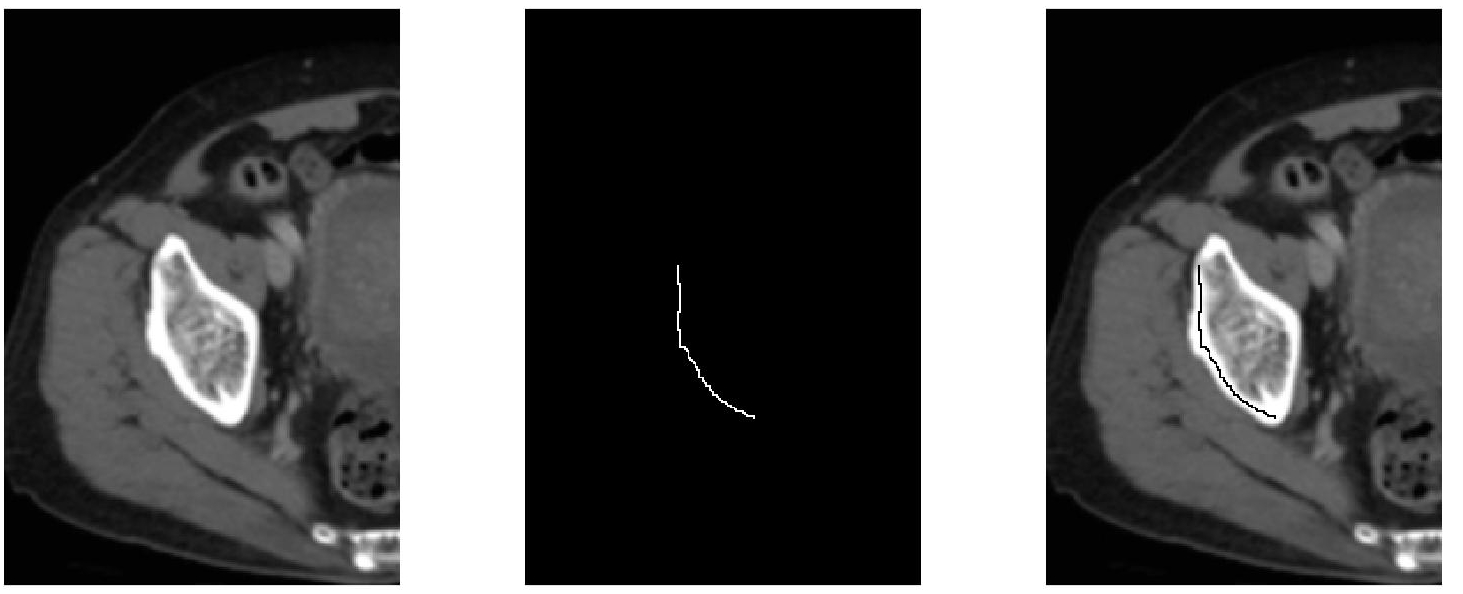
\includegraphics[width = 16cm]{p1_1.jpg}
	\caption{Result for scissors algorithm}
\end{figure}

\begin{figure}[!htbp]
	\centering
	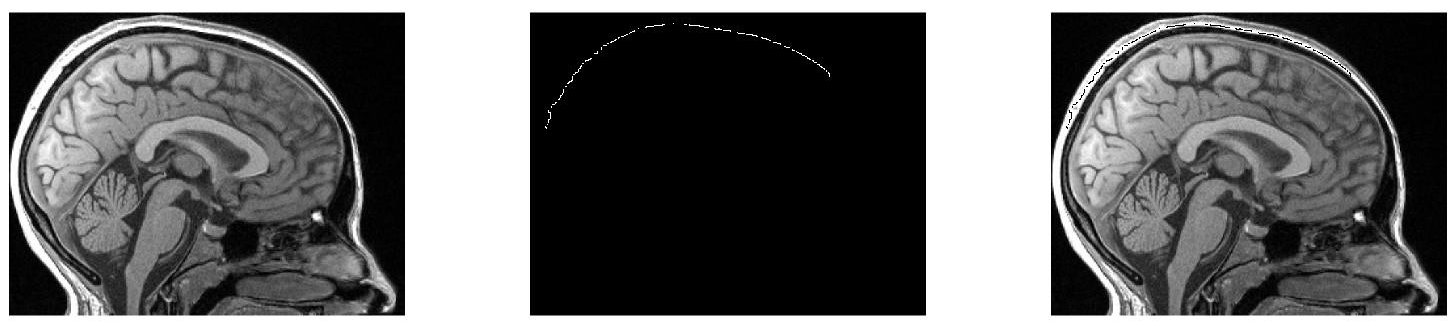
\includegraphics[width = 16cm]{p1_2.jpg}
	\caption{Result for scissors algorithm}
\end{figure}



\newpage

\section{Problem 2}

\subsection{Part 1}

I use the hough transform of with paramets $d$ and $\theta$:  $xcos\theta - ysin\theta = d$.
The resolution for d is 1 and 1 degree for $\theta$.
Some results are shown in Figure 2.1 - 2.3.

\begin{figure}[!htbp]
	\centering
	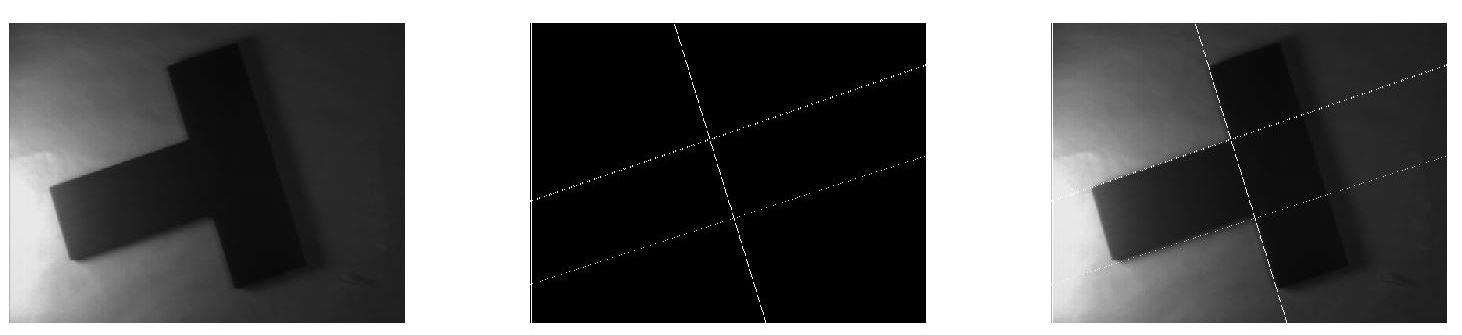
\includegraphics[width = 16cm]{p2_1.jpg}
	\caption{Result for hough transform}
\end{figure}
\begin{figure}[!htbp]
	\centering
	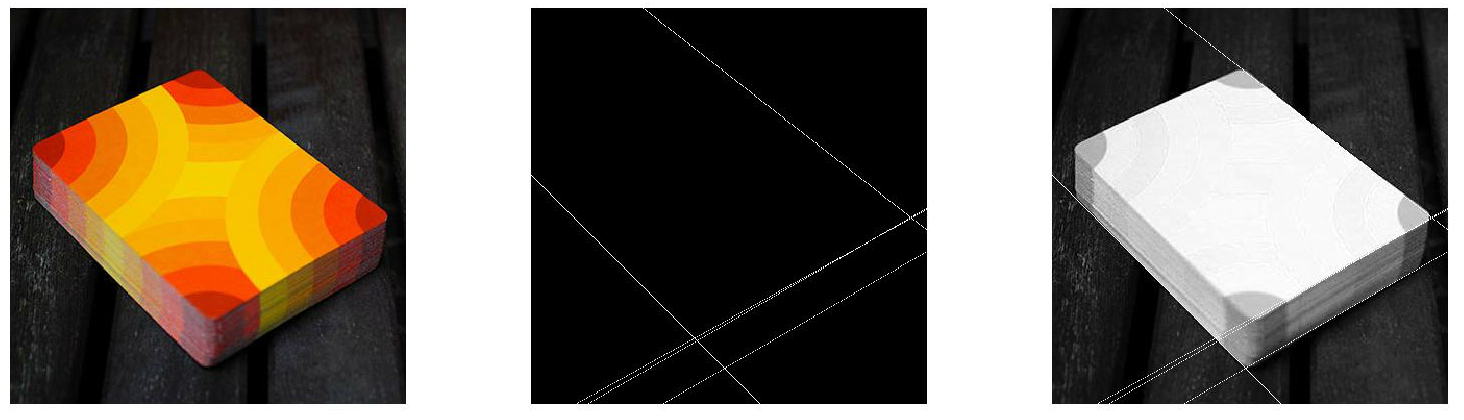
\includegraphics[width = 16cm]{p2_2.jpg}
	\caption{Result for hough transform}
\end{figure}
\begin{figure}[!htbp]
	\centering
	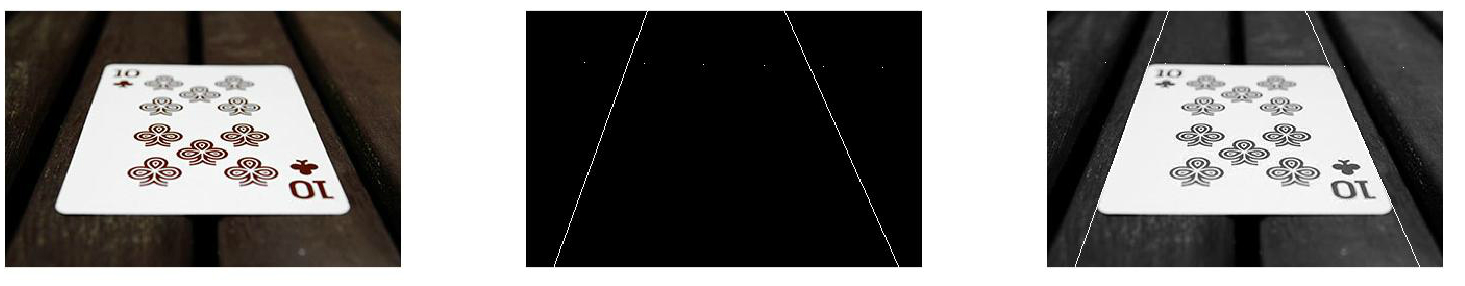
\includegraphics[width = 16cm]{p2_3.jpg}
	\caption{Result for hough transform}
\end{figure}

\subsection{Part 2}

Two reference points are (21, 118) and (32, 11).
\\

In myHoughCircleTrain part, I store the relative position between center point and boundary point.
That is, (center x - boundary x,  center y - boundary y).
Then in myHoughCircleTest method, for every boundary points, I mark the all possible center points
by (relative x + boundary x,  relative y + boundary y).
Select the max two points in the hough space as the reference points.


\begin{figure}[!htbp]
	\centering
	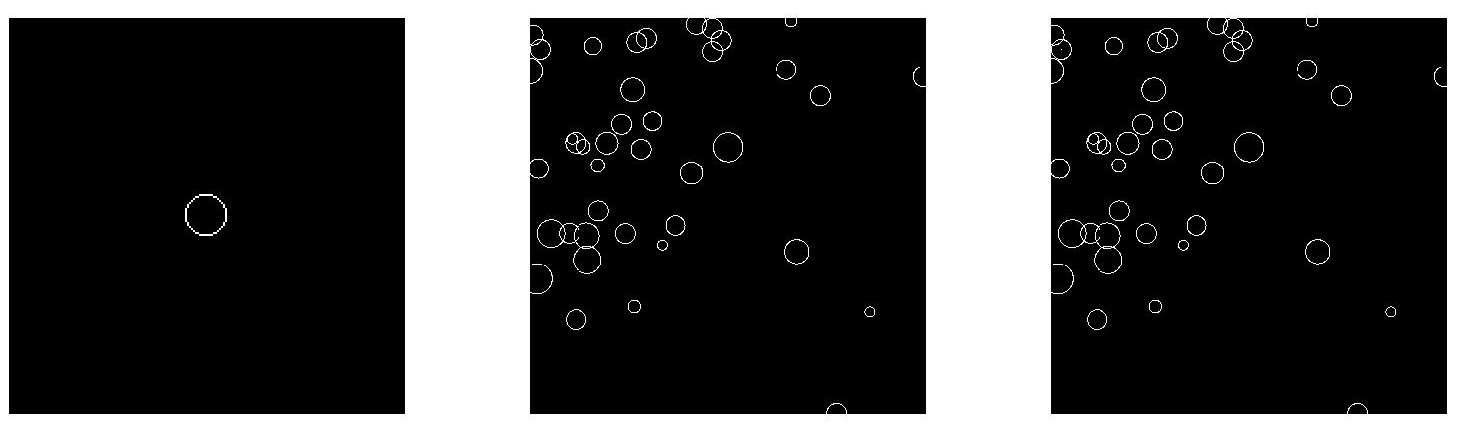
\includegraphics[width = 16cm]{p2_4.jpg}
	\caption{Result for circle finding, the reference points are marked in the third figure}
\end{figure}

\newpage


\section{Problem 3}

I use the dynamic programming method to get minimum energy for each iteration.
I can get the best result with alpha=0.3 and beta=0.5. 
In gerneral, I found the more points I use, the better result I can get.
I use about 50 points for the following results.
The best result is shown in Figure 3.1 and Figure 3.2.
\\

If the alpha is a little larger, say alpha=1, The result may be not optimal. From Figure 3.3, we can see that the snake shrink too much on the top part of the region.
\\

If the alpha and beta is too large, such as alpha=10 and beta=10, the snake will shrink to a cluster. This is shown in Figure 3.4.
\\

If the alpha and beta is too small, the snake will go along with the other boundary in the figure. This is shown in Figure 3.5.
\\

If the number of points is too small, the result will be very bad. 
This is shown in Figure 3.6, with alpha=0.5 ,beta=1 and 10 points.
\\

\begin{figure}[!htbp]
	\centering
	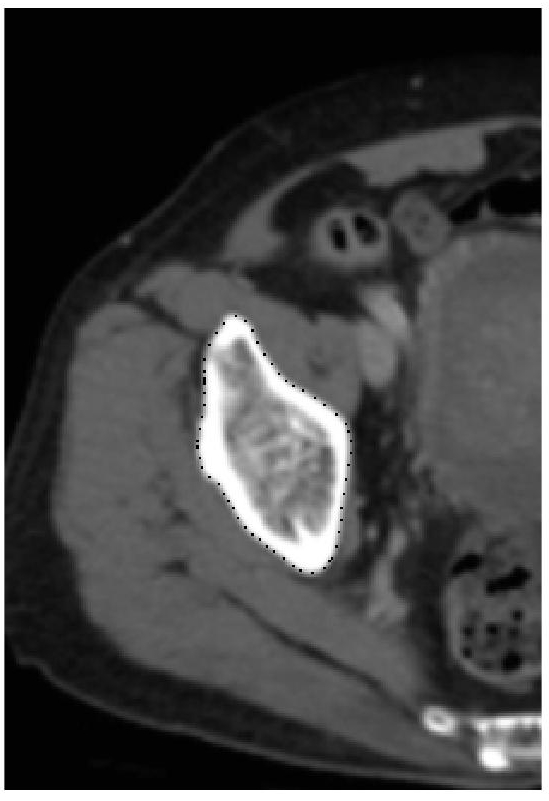
\includegraphics[width = 12cm]{p3_1.jpg}
	\caption{Final result with alpha=0.3 and beta=0.5}
\end{figure}


\begin{figure}[!htbp]
	\centering
	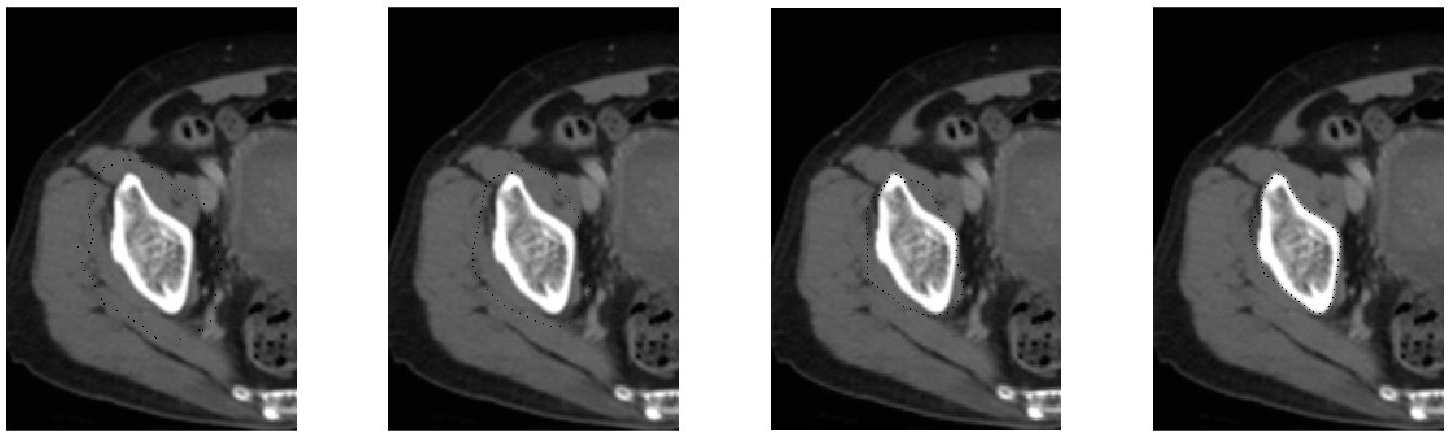
\includegraphics[width = 16cm]{p3_2.jpg}
	\caption{Result after every 10 steps with alpha=0.5 and beta=1}
\end{figure}



\begin{figure}[!htbp]
	\centering
	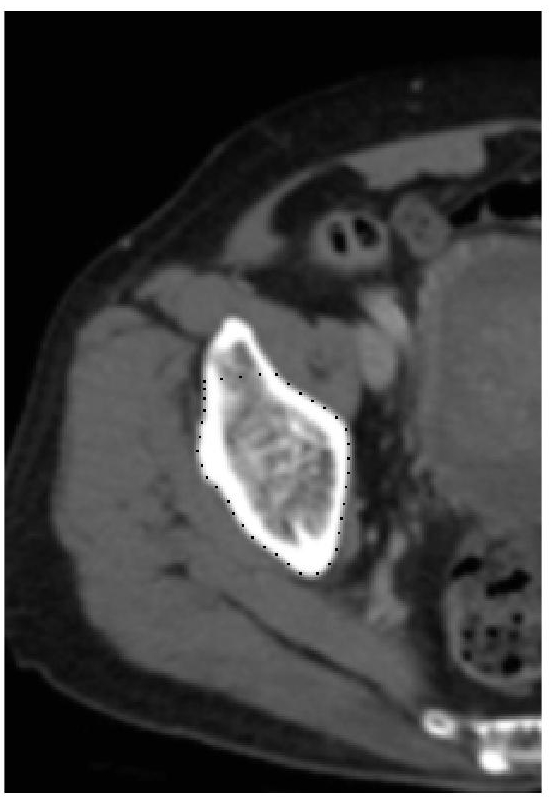
\includegraphics[width = 12cm]{p3_3.jpg}
	\caption{Final result with alpha=1 and beta=1, shrink too much on the top part of the region}
\end{figure}



\begin{figure}[!htbp]
	\centering
	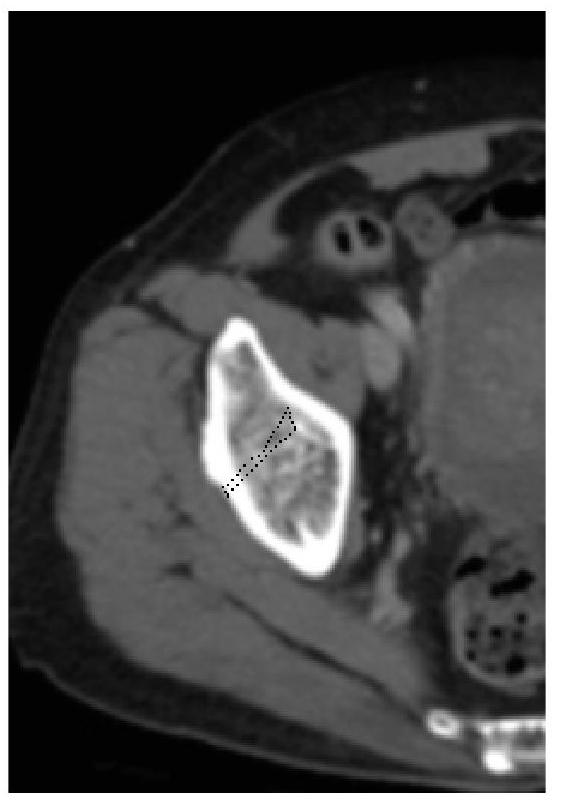
\includegraphics[width = 12cm]{p3_4.jpg}
	\caption{Final result with alpha=10 and beta=10, shrink to a cluster}
\end{figure}


\begin{figure}[!htbp]
	\centering
	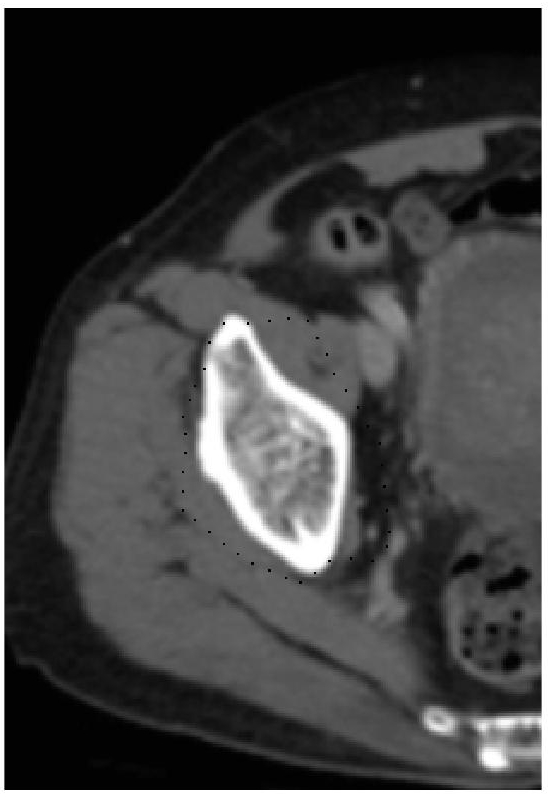
\includegraphics[width = 12cm]{p3_5.jpg}
	\caption{Final result with alpha=0.05 and beta=0.05, snake get on the other boudary}
\end{figure}


\begin{figure}[!htbp]
	\centering
	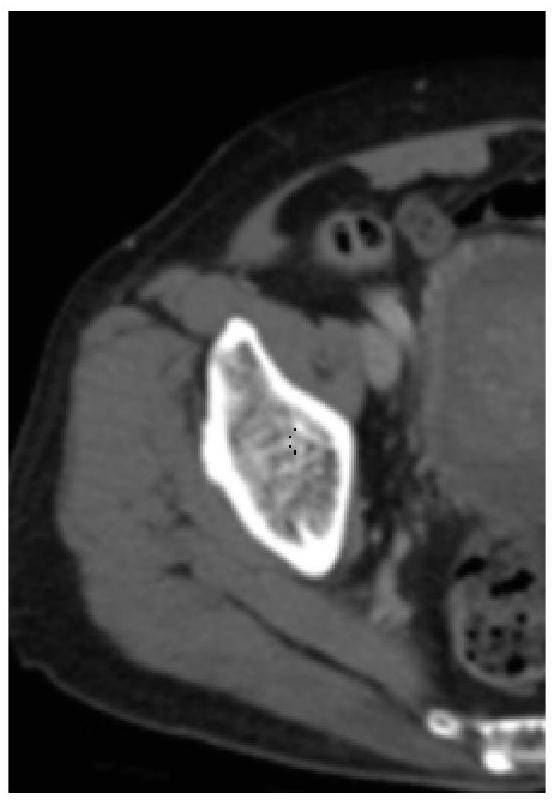
\includegraphics[width = 12cm]{p3_6.jpg}
	\caption{Final result with alpha=0.5 ,beta=1 and only 10 points}
\end{figure}



%----------------------------------------------------------------------------------------

\end{document}
